%% Robust Level-3 Autonomous Drone Racing by Gate Search and Time-Optimal MPCC
%% Report v4: built around controller_v24_r10 (blind spiral gate search + v10.5 MPCC).
%% v4 corrects final.toml (randomized graded track, reveals nominal within 15 cm; not fixed) and its numbers;
%% adds a No-Search Variant subsection (search stays the headline).
%% Built on the IEEE conference template (IEEEtran).
%% External image files live in figs_v24_r10/ (fig_topdown.png, fig_3d.png, fig_speed.png).
%% The gate-weight schedule and all other diagrams are self-contained TikZ.
%% Compile with pdflatex, run twice.
\documentclass[conference]{IEEEtran}
\IEEEoverridecommandlockouts
% The preceding line is only needed to identify funding in the first footnote. If that is unneeded, please comment it out.
\usepackage{cite}
\usepackage{url}
\usepackage{amsmath,amssymb,amsfonts}
\usepackage{algorithm}
\usepackage{algorithmic}
\usepackage{graphicx}
\graphicspath{{figs_v24_r10/}}
\usepackage{textcomp}
\usepackage{xcolor}
\usepackage{tikz}
\usetikzlibrary{arrows.meta,positioning,calc,shapes.geometric}
\def\BibTeX{{\rm B\kern-.05em{\sc i\kern-.025em b}\kern-.08em
    T\kern-.1667em\lower.7ex\hbox{E}\kern-.125emX}}

\begin{document}

\title{Robust Level~3 Autonomous Drone Racing\\ by Gate Search and Time-Optimal Contouring Control}

\author{\IEEEauthorblockN{1\textsuperscript{st} Ahmet Arda Hız}
\IEEEauthorblockA{\textit{Learning Systems and Robotics} \\
\textit{Technical University of Munich}\\
Munich, Germany \\
aarda.hiz@tum.de}
\and
\IEEEauthorblockN{2\textsuperscript{nd} Deniz \"Ozt\"urk}
\IEEEauthorblockA{\textit{Learning Systems and Robotics} \\
\textit{Technical University of Munich}\\
Munich, Germany \\
deniz.oeztuerk@tum.de}
}

\maketitle

\begin{abstract}
Autonomous drone racing tests a controller at the limit of a vehicle's dynamics. The competition is staged as a ladder of difficulty levels, and we advanced through all of them. Level 3 is the last and hardest, so it is the focus of this report and the capstone of the project, since it needs the racing foundation that the earlier levels build. We study this full Level 3 setting, where the gate positions and the gate order are randomized and the true pose of an object is revealed only when the drone comes within 0.7~m of it. A controller that reads the nominal layout does not transfer to this setting, so our controller first finds the gates and then races them. It does not use the nominal positions at all. It flies a fixed spiral sweep that climbs above the obstacles and covers the arena, and each gate is discovered when the drone passes within sensor range in the horizontal plane. The discovered gates are handed to a time-optimal Model Predictive Contouring Control (MPCC) stage that races them, with a gate-aware contouring weight and a dynamics-aware progress anchor for reliability. The method is general. In its robust setting it finishes 12 of 20 runs on randomized Level 3 tracks at a lap time of 18.8~s, and 9 of 20 runs on the randomized \texttt{final.toml} competition track at 26.9~s. A faster, more aggressive setting of the same controller cuts the Level 3 lap time to 12.8~s at a small cost in success rate. We describe the design, the price the search pays for generality, and how it grew out of a fast known-track racing core that we flew on the real drone at 9.55~s.
\end{abstract}

\section{Introduction}
Autonomous drone racing asks a controller to fly a quadrotor through a set of gates in the shortest time without hitting a gate frame or an obstacle. It is a common benchmark because a fast lap forces the vehicle to work near its actuation limit, where small errors are punished at once \cite{survey}. Much of the drone racing work assumes a known track, where every gate position is fixed before the flight and the task is a single time-optimal trajectory \cite{foehn,minsnap}. The full Level 3 setting breaks that assumption. The gate positions and the gate order are randomized, and the vehicle only sees the true geometry once it is close.

This report comes out of a course project built as a ladder of levels, where each level switches on more disturbance than the one below. We worked through the lower levels first, on a known track and then under inertial and pose randomization, and each result carried into the next, so the top of the ladder reuses a racing core that the lower levels validated. Level 3 is that top. It randomizes the whole layout, which makes it the hardest and most general level and the end product of the project. The graded evaluation runs on a shared configuration, \texttt{final.toml}, with a fixed seed, so all groups are compared on the same randomized draw. We treat it as one more Level 3 draw and never read its revealed nominal layout, which is what our design is built to do.

We study the Level 3 setting of the LSY Drone Racing competition. Gate and obstacle positions are drawn at random, and the true pose of an object is reported only when the drone is within 0.7~m of it. A controller that relies on the nominal layout therefore does not work here, because the layout it would read is not the one it flies. Our controller does not read the nominal layout at all. It finds the gates by flying and racing them once they are found.

The controller has two phases. First it searches. It flies a fixed spiral that climbs above the obstacles and sweeps the arena, and a gate is discovered when the drone passes within sensor range of it. Then it races. The discovered gates are handed to a time-optimal Model Predictive Contouring Control (MPCC) stage \cite{mpcc,lam} that treats path progress as a state and traversal speed as an output, so speed is an outcome of the optimization. The contribution of this report is that controller and the design choices that make it robust on any Level 3 layout.
\begin{itemize}
\item A blind gate search that finds every gate without the nominal positions, so the same controller works on any randomized layout.
\item A gate-aware contouring weight and a dynamics-aware progress anchor that keep the racing stage reliable once the gates are known.
\end{itemize}
We evaluate the controller on randomized Level 3 tracks and on the randomized competition track, and we relate it to a fast known-track racing core that we flew on the real Crazyflie at 9.55~s.

\section{Related Work}
\label{sec:related}
Time-optimal quadrotor flight through a fixed set of gates is well studied. Foehn et al.\ compute a full time-optimal trajectory that respects the single-rotor thrust limits \cite{foehn}, and minimum-snap trajectories \cite{minsnap} are a common lighter planning choice. These methods give the fastest known laps on a known track, but they assume the gates are known and do not move.

MPCC was introduced for machining \cite{lam} and brought to racing on 1:43 cars \cite{liniger}. Romero et al.\ applied a time-optimal MPCC to quadrotor flight and showed it reaches the actuator limit in real time \cite{mpcc}. MPCC++ adds a safe tunnel around the reference as hard constraints \cite{mpccpp}. We use the time-optimal MPCC formulation for the racing stage.

Learning-based controllers train a policy that maps the observation to an action in one forward pass and have reached champion-level lap times \cite{champion,songrl}. They are fast but need training and are harder to inspect. The part that is specific to Level 3 is that the gates are not known in advance, so the controller has to discover them before it can race. We handle this with an explicit search stage rather than a learned exploration policy.

\section{Problem Description}
\label{sec:problem}
We use the LSY Drone Racing environment, which builds on the safe-control-gym benchmark \cite{scg} with a Crazyflie 2.1 quadrotor \cite{crazyflie} as the model. The vehicle has a mass of 43~g and a thrust-to-weight ratio near 1.9. A track holds four gates and four obstacles. A gate opening is 0.4~m wide inside a 0.72~m frame, so the usable gap is about three vehicle widths.

At each step the controller reads an observation
\begin{equation}
o = [\, p,\; v,\; q,\; G,\; O,\; i \,],
\label{eq:obs}
\end{equation}
with position $p \in \mathbb{R}^3$, velocity $v \in \mathbb{R}^3$, orientation quaternion $q$, the gate poses $G$, the obstacle positions $O$ and the index $i$ of the next gate. A gate starts at a nominal pose and switches to its true pose once the drone is within the 0.7~m sensor range. The reveal test uses the horizontal distance between the drone and the gate center, so altitude does not matter for detection. In the lab the true poses come from an external motion capture system (Vicon), which tracks reflective markers on the gates and obstacles. The command is sent at 50~Hz. The environment runs in attitude mode, so the output is
\begin{equation}
a = [\, \phi,\; \theta,\; \psi,\; f \,],
\label{eq:act}
\end{equation}
a roll, pitch and yaw with a collective thrust $f$. An onboard controller at 500~Hz tracks $a$.

The challenge is a ladder of difficulty levels that differ by which disturbances are active. Level 0 has no disturbance. The drone and the full track are known, so it measures raw speed. Level 1 randomizes the drone's inertial properties (mass and inertia) and its start pose, while the track stays known. Level 2 also randomizes the gate and obstacle poses within set bounds, revealed within the sensor range, on a layout that is otherwise fixed. Level 3 randomizes the layout itself, so the gate positions and the gate order change every run, which forces the controller to plan online in flight. This is the setting we target. The graded evaluation uses a separate configuration, \texttt{final.toml}, released in the last lab session. Like Level 3 it randomizes the whole layout, but with a fixed seed, so every group flies the same draw and the lap times compare directly. It keeps the drone and pose disturbances and reveals each gate and obstacle within 0.7~m, with the reported nominal pose already within 15~cm of the truth. We report on it as well, but our controller stays a general Level 3 policy. It does not read the nominal layout of any track, so even when a nominal prior is available it runs the same blind search instead of exploiting it.

Two features of the setting drive the design. The layout is unknown, so the controller cannot fly straight to a gate; it has to find it first. And a gate is seen late, so once the layout is known the racing stage still has to correct for the last few centimeters of a revealed pose within a short window.

\section{Methodology}
\label{sec:method}

\subsection{Overview}
The controller runs three phases. A short, aggressive launch, which we call the fast launch, climbs off the pad in a fixed brief window instead of a slow hover takeoff, then it enters the search and race loop of Fig.~\ref{fig:pipeline}. In the search phase it sweeps the arena and discovers the gates. In the race phase it hands the discovered gates to a time-optimal MPCC that flies through them and returns a world-frame acceleration, which an attitude stage turns into a thrust and attitude command. The loop runs at 50~Hz. Nothing in the controller reads the nominal layout, so the same phases run on any Level 3 track.

\begin{figure}[t]
\centering
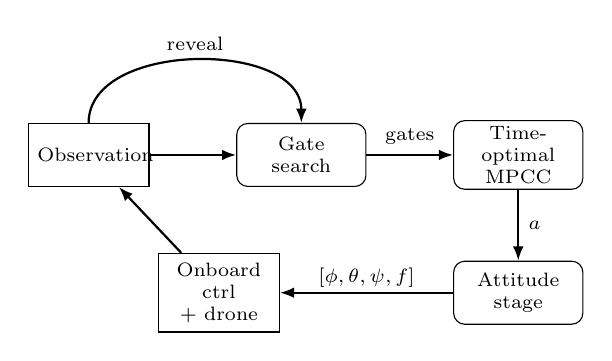
\begin{tikzpicture}[
  node distance=6mm and 11mm,
  block/.style={draw, rounded corners, align=center, minimum height=8mm, inner sep=2pt, font=\scriptsize, text width=15mm},
  io/.style={draw, align=center, font=\scriptsize, text width=13mm, minimum height=8mm},
  arr/.style={-{Latex[length=1.8mm]}, thick}
]
\node[io] (obs) {Observation};
\node[block, right=of obs] (search) {Gate\\ search};
\node[block, right=of search] (mpcc) {Time-optimal\\ MPCC};
\node[block, below=9mm of mpcc] (att) {Attitude\\ stage};
\node[io, left=22mm of att] (drone) {Onboard ctrl\\ + drone};
\draw[arr] (obs) -- (search);
\draw[arr] (search) -- node[above, font=\scriptsize]{gates} (mpcc);
\draw[arr] (mpcc) -- node[right, font=\scriptsize]{$a$} (att);
\draw[arr] (att) -- node[midway, above, font=\scriptsize, fill=white, inner sep=1.5pt]{$[\phi,\theta,\psi,f]$} (drone);
\draw[arr] (drone) -- (obs);
\draw[arr] (obs.north) to[out=90,in=90] node[above, font=\scriptsize]{reveal} (search.north);
\end{tikzpicture}
\caption{Controller structure after takeoff. The drone reads the observation, the search discovers the gates, a time-optimal MPCC races them and the attitude stage produces the command. A gate is revealed when the drone passes within 0.7~m of it.}
\label{fig:pipeline}
\end{figure}

\subsection{Finding the Gates: Spiral Search}
\label{sec:search}
On Level 3 the gate positions and the gate order are unknown, so the controller must find the gates before it can race. It does this with a fixed geometric sweep and does not use the nominal positions. After takeoff the drone climbs to a search altitude of 1.8~m, which is above the 1.52~m obstacle poles, so the sweep cannot hit one. It then follows an Archimedean spiral that grows outward from its start position, with a radial step of 0.6~m out to a radius of 2.2~m, clipped to the arena, flown at 1.1~m/s with a PD tracker. Fig.~\ref{fig:spiral} sketches the sweep.

\begin{figure}[t]
\centering
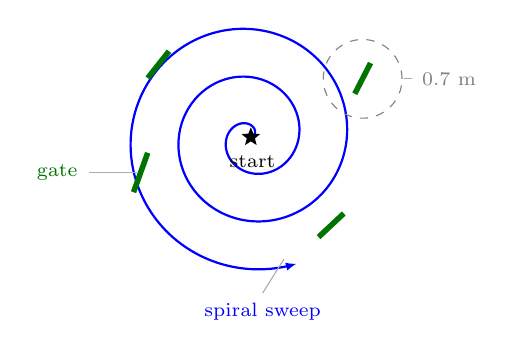
\begin{tikzpicture}[scale=1.0, font=\scriptsize,
  gate/.style={green!45!black, line width=2pt},
  lead/.style={gray!65, line width=0.4pt}]
  % Archimedean spiral sweep; the arrowhead marks the outward direction
  \draw[blue, thick, -{Latex[length=1.4mm]}]
        plot[domain=0:1010, samples=240, smooth]
        ({0.0017*\x*cos(\x)}, {0.0017*\x*sin(\x)});
  % start marker (star, matching the top-down figure)
  \node[star, star point ratio=2.3, minimum size=6pt, inner sep=0pt,
        fill=black, draw=black] at (0,0) {};
  \node[anchor=north, inner sep=2.5pt] at (0.02,-0.14) {start};
  % gates as green openings (same color convention as the racing-line figure)
  \draw[gate] (-1.31,0.75) -- (-1.04,1.09);
  \draw[gate] ( 1.32,0.55) -- ( 1.52,0.94);
  \draw[gate] ( 0.86,-1.27) -- ( 1.18,-0.97);
  \draw[gate] (-1.49,-0.70) -- (-1.31,-0.20);
  % sensor reveal radius on one gate; the spiral crosses it, so the gate is found
  \draw[gray, dashed] (1.42,0.74) circle (0.5);
  % labels sit outside the swept disk with short leaders, so nothing overlaps
  \node[gray, anchor=west] (rl) at (2.05,0.74) {0.7~m};
  \draw[lead] (rl.west) -- (1.94,0.74);
  \node[gate, anchor=east] (gl) at (-2.05,-0.45) {gate};
  \draw[lead] (gl.east) -- (-1.44,-0.45);
  \node[blue, anchor=north] (sl) at (0.15,-1.98) {spiral sweep};
  \draw[lead] (sl.north) -- (0.42,-1.55);
\end{tikzpicture}
\caption{Blind gate search, seen from above. The drone climbs above the obstacle poles and follows a fixed Archimedean spiral that covers the arena. Each gate (green) is revealed when the spiral passes within 0.7~m of its center in the horizontal plane, drawn as the dashed circle on one gate.}
\label{fig:spiral}
\end{figure}

As the drone's horizontal position comes within the 0.7~m sensor range of a gate center, that gate is revealed and its index is collected. The search ends when every gate has been discovered or the spiral is finished, as in Fig.~\ref{fig:search}. The discovered true poses are then passed to the racing stage. The sweep is blind by design. It covers the arena geometrically, so it works on any layout, and it is the price the controller pays for not knowing where the gates are.


\begin{figure}[t]
\centering
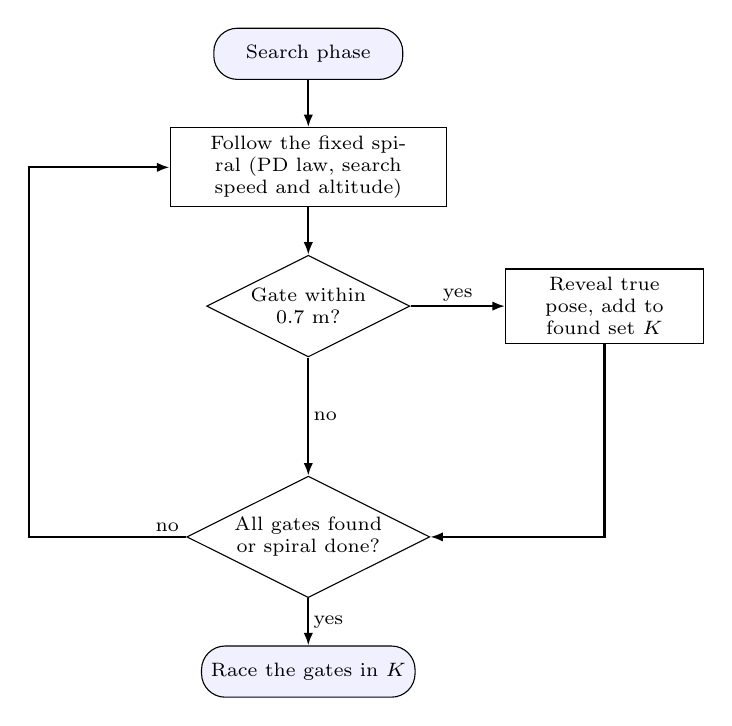
\begin{tikzpicture}[
  font=\scriptsize,
  node distance=6mm and 12mm,
  term/.style={draw, rounded corners=3mm, align=center, minimum width=24mm, minimum height=6.5mm, fill=blue!6},
  proc/.style={draw, align=center, text width=33mm, minimum height=8mm, inner sep=3pt},
  dec/.style={draw, diamond, aspect=2, align=center, inner sep=1pt},
  flow/.style={-{Latex[length=1.6mm]}, thick},
  lbl/.style={inner sep=1.5pt}
]
\node[term] (start) {Search phase};
\node[proc, below=of start] (follow) {Follow the fixed spiral (PD law, search speed and altitude)};
\node[dec, below=of follow] (near) {Gate within\\ 0.7~m?};
\node[proc, right=12mm of near, text width=23mm] (reveal) {Reveal true pose, add to found set $K$};
\node[dec, below=15mm of near] (done) {All gates found\\ or spiral done?};
\node[term, below=of done] (race) {Race the gates in $K$};

\draw[flow] (start) -- (follow);
\draw[flow] (follow) -- (near);
\draw[flow] (near) -- node[lbl, above]{yes} (reveal);
\draw[flow] (reveal) |- (done);
\draw[flow] (near) -- node[lbl, right]{no} (done);
\draw[flow] (done) -- node[lbl, right]{yes} (race);
\draw[flow] (done.west) -- node[lbl, above, pos=0.12]{no} ++(-2.0,0) |- (follow.west);
\end{tikzpicture}
\caption{Gate search, run once per control tick in the search phase. The drone follows the fixed spiral and reveals any gate that comes within 0.7~m in the horizontal plane, adding it to the found set $K$. It keeps sweeping until every gate is found or the spiral ends, then hands $K$ to the racing stage.}
\label{fig:search}
\end{figure}

\subsection{Time-Optimal MPCC}
\label{sec:mpcc}
Once the gates are known the racing stage is a time-optimal MPCC problem \cite{mpcc,lam}. A planner fits a clamped cubic spline through the discovered gates, with two virtual columns per gate at the frame edges so the spline threads the opening center, and a keep-out radius around the obstacles. MPCC adds a progress variable $\xi$ that runs along this path and a progress rate $v_\xi$. The state is
\begin{equation}
x = [\, p^\top,\; v^\top,\; \xi,\; v_\xi \,]^\top,
\end{equation}
with control acceleration $a$ and progress acceleration $u_\xi$ and a double-integrator model,
\begin{equation}
\dot p = v,\quad \dot v = a,\quad \dot\xi = v_\xi,\quad \dot v_\xi = u_\xi .
\end{equation}
The reference is linearized around a predicted progress $\bar\xi$ with tangent $t(\bar\xi)$, and the path error splits into a lag part along the tangent and a contouring part across it (Fig.~\ref{fig:contour}),
\begin{equation}
e = p - \big(p_{\text{ref}}(\bar\xi) + t(\bar\xi)(\xi-\bar\xi)\big),\quad e_l = e^\top t,\quad e_c = e - e_l\,t .
\end{equation}
The stage cost trades path accuracy against time,
\begin{equation}
\ell = q_c(\xi)\,\lVert e_c \rVert^2 + w_l\, e_l^2 - \mu\, v_\xi + w_a \lVert a \rVert^2 + r_v\, u_\xi^2 .
\label{eq:cost}
\end{equation}
The term $-\mu\, v_\xi$ rewards progress, so the solver flies as fast as the constraints allow, and $q_c(\xi)$ is a per-stage weight (Section~\ref{sec:gateweight}). The actuator limits enter as constraints on the commanded thrust $f = a + g$,
\begin{equation}
\lVert f \rVert^2 \le a_{\max}^2, \quad f_z \ge a_{z,\min}, \quad (\kappa_t f_z)^2 \ge f_x^2 + f_y^2,
\end{equation}
the thrust magnitude, a minimum lift and a tilt limit. A friction-circle curvature cap completes the set,
\begin{equation}
v_{\text{curv}}(\xi) = \mathrm{clip}\!\left(\sqrt{a_{\text{lat}}/\kappa(\xi)},\; v_{\min},\; v_{\max}\right),
\label{eq:curv}
\end{equation}
which soft-bounds the speed and the progress rate. We solve the program in real time with acados \cite{acados} using a sequential quadratic programming real-time iteration \cite{rti}, with the quadratic programs handled by HPIPM \cite{hpipm}. The horizon is 18 steps at 0.05~s, and the first acceleration of the horizon is the command.

\begin{figure}[t]
\centering
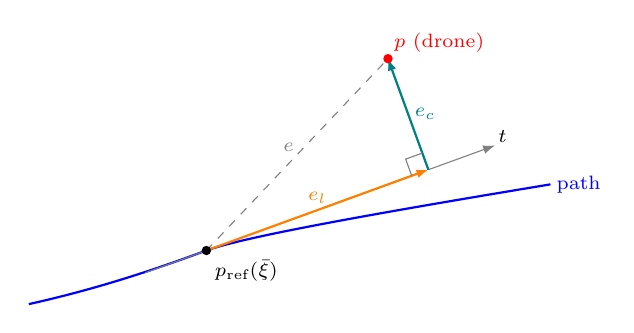
\begin{tikzpicture}[scale=1.5, font=\scriptsize,
  ar/.style={-{Latex[length=1.5mm]}},
  dot/.style={circle, fill=black, inner sep=1.2pt}]
  % Precomputed points: tangent at 20 deg, normal at 110 deg.
  % F = P + 2.0*tangent (foot);  D = F + 1.0*normal (drone).
  \coordinate (P) at (0,0);
  \coordinate (F) at (1.879,0.684);
  \coordinate (D) at (1.537,1.624);
  % path: tangent to the 20 deg direction at P (control handles kept along it)
  \draw[blue, thick]
     (-1.504,-0.454)
     .. controls (-0.846,-0.308) and (-0.329,-0.120) .. (P)
     .. controls (0.329,0.120) and (1.504,0.327) .. (2.913,0.560);
  \node[blue, anchor=west, inner sep=2pt] at (2.913,0.560) {path};
  % tangent line: stub before P, then continues past the foot with the t arrow
  \draw[gray] (-0.517,-0.188) -- (P);
  \draw[gray, ar] (F) -- (2.443,0.889) node[black, anchor=south west, inner sep=1pt] {$t$};
  % error decomposition: right triangle ref (P) -- foot (F) -- drone (D)
  \draw[orange, thick, ar] (P) -- (F) node[midway, above, inner sep=2pt] {$e_l$};
  \draw[teal, thick, ar]   (F) -- (D) node[midway, right, inner sep=2pt] {$e_c$};
  \draw[gray, dashed]      (P) -- (D) node[midway, above left, inner sep=1pt] {$e$};
  % right-angle mark at the foot
  \draw[gray] (1.738,0.633) -- (1.687,0.774) -- (1.828,0.825);
  % points and labels
  \node[dot] at (P) {};
  \node[anchor=north west, inner sep=2pt] at (0.02,-0.03) {$p_{\text{ref}}(\bar\xi)$};
  \node[dot, fill=red] at (D) {};
  \node[red, anchor=south west, inner sep=2pt] at (D) {$p$ (drone)};
\end{tikzpicture}
\caption{Contouring geometry. At the reference point $p_{\text{ref}}(\bar\xi)$ the path has tangent $t$. The error from the drone position $p$ splits into a lag part $e_l$ along $t$ and a contouring part $e_c$ across it, and the two meet at a right angle at the foot. Together they form the full error $e$. MPCC penalizes the contouring error hard and the lag softly, and rewards progress so the drone flies as fast as the constraints allow.}
\label{fig:contour}
\end{figure}

\subsection{Gate-Aware Contouring Weight}
\label{sec:gateweight}
A single contouring weight is wrong somewhere on the track. High everywhere brakes the vehicle on the straights, and low everywhere lets it drift at a gate, where a drift is a miss. We make the weight a function of progress,
\begin{equation}
q_c(\xi) = q_{\text{base}} + q_{\text{gate}} \sum_j \exp\!\left(-\frac{(s(\xi)-s_j)^2}{2\sigma^2}\right),
\label{eq:weight}
\end{equation}
with $s_j$ the arc position of gate $j$ and $\sigma$ the window width. The weight is low between gates and peaks at each gate, shown in Fig.~\ref{fig:weight}. The vehicle is held on the line where a gate must be threaded and runs free elsewhere, which lets the speed rise without a drop in the gate pass rate.

\begin{figure}[t]
\centering
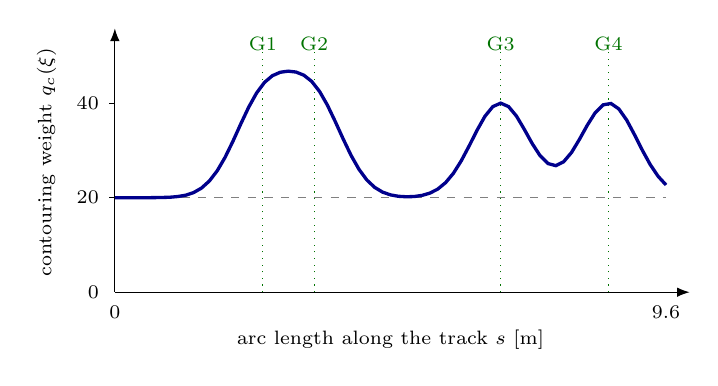
\begin{tikzpicture}[x=1cm,y=1cm,every node/.style={font=\scriptsize}]
  % gate guide lines and labels
  \foreach \gx/\gl in {1.88/G1, 2.53/G2, 4.90/G3, 6.27/G4}{%
    \draw[green!45!black,dotted] (\gx,0) -- (\gx,3.05);
    \node[green!45!black,anchor=south] at (\gx,2.95) {\gl};
  }
  % baseline
  \draw[gray,dashed] (0,1.2) -- (7,1.2);
  % axes
  \draw[-{Latex[length=1.6mm]}] (0,0) -- (7.3,0);
  \draw[-{Latex[length=1.6mm]}] (0,0) -- (0,3.35);
  % y ticks
  \draw (0,1.2) -- (-0.08,1.2) node[anchor=east] {20};
  \draw (0,2.4) -- (-0.08,2.4) node[anchor=east] {40};
  \node[anchor=east] at (-0.08,0) {0};
  % x ticks
  \node[anchor=north] at (0,-0.05) {0};
  \node[anchor=north] at (7,-0.05) {9.6};
  % axis labels
  \node[anchor=north] at (3.5,-0.35) {arc length along the track $s$ [m]};
  \node[rotate=90,anchor=south] at (-0.62,1.65) {contouring weight $q_c(\xi)$};
  % weight schedule q_c(xi) = q_base + q_gate * sum_j exp(-(s(xi)-s_j)^2 / 2 sigma^2)
  \draw[very thick,blue!55!black] plot coordinates {(0.000,1.200) (0.100,1.200) (0.200,1.200) (0.300,1.200) (0.400,1.200) (0.500,1.201) (0.600,1.203) (0.700,1.206) (0.800,1.215) (0.900,1.232) (1.000,1.265) (1.100,1.322) (1.200,1.412) (1.300,1.542) (1.400,1.713) (1.500,1.918) (1.600,2.139) (1.700,2.350) (1.800,2.530) (1.900,2.664) (2.000,2.749) (2.100,2.793) (2.200,2.807) (2.300,2.796) (2.400,2.756) (2.500,2.677) (2.600,2.549) (2.700,2.374) (2.800,2.165) (2.900,1.945) (3.000,1.737) (3.100,1.561) (3.200,1.425) (3.300,1.331) (3.400,1.271) (3.500,1.236) (3.600,1.218) (3.700,1.212) (3.800,1.215) (3.900,1.229) (4.000,1.258) (4.100,1.309) (4.200,1.391) (4.300,1.511) (4.400,1.670) (4.500,1.859) (4.600,2.057) (4.700,2.234) (4.800,2.357) (4.900,2.401) (5.000,2.357) (5.100,2.237) (5.200,2.068) (5.300,1.888) (5.400,1.734) (5.500,1.634) (5.600,1.607) (5.700,1.657) (5.800,1.775) (5.900,1.941) (6.000,2.121) (6.100,2.279) (6.200,2.379) (6.300,2.397) (6.400,2.328) (6.500,2.186) (6.600,1.999) (6.700,1.801) (6.800,1.619) (6.900,1.471) (7.000,1.362)};
\end{tikzpicture}
\caption{The gate-aware contouring weight along the track, computed from \eqref{eq:weight} for the competition layout. The weight sits at a low base on the straights and rises to a peak at each gate (G1 to G4), so tracking is stiff only where a gate must be threaded. Gates whose arc positions fall within the window merge into a single wider peak.}
\label{fig:weight}
\end{figure}

\subsection{Dynamics-Aware Progress Anchor}
\label{sec:anchor}
The MPCC needs a value of the progress $\xi$ each step. The direct choice, the arc length of the nearest path point, fails at a hairpin, where the path folds back and a far leg comes close in space, so the nearest-point search jumps to it and skips a gate. We anchor the progress to the solver's own predicted progress one step ahead, which advances at the bounded rate $v_\xi$ and cannot jump, and correct it with a nearest-point search limited to a band around the prediction. The far leg of a fold lies outside the band and is never selected, while the gate motion lies inside it. The anchor removes the fold skip without changing tracking elsewhere.

\subsection{Two Settings}
\label{sec:settings}
We use two settings of the same controller. Both run the same blind search and the same MPCC, and neither reads the nominal layout, so the difference is aggressiveness and not method. The robust setting is for randomized Level 3. It keeps a moderate speed budget so that it finishes on as many random draws as possible. The fast setting is more aggressive. It raises the MPCC speed budget and tightens the search, so it reaches the gates sooner and races them harder. On Level 3 it cuts the lap time by about a third, from 18.8~s to 12.8~s, at a small cost in success rate. The two settings differ only in these parameters, so this is an aggressiveness choice and not a change of method. Table~\ref{tab:results} reports both settings.

\section{Evaluation and Results}
\label{sec:results}

\subsection{Setup}
We evaluate the controller on randomized Level 3 tracks with the Level 3 evaluation script, and on the randomized competition configuration (\texttt{final.toml}) with the provided seed. Fig.~\ref{fig:racingline} shows a lap on a \texttt{final.toml} draw. Both settings use at least 20 runs. The controller reads no nominal layout in either case, and the search parameters and the MPCC weights are shared across all tracks. Table~\ref{tab:params} lists the main parameters.

\begin{table}[htbp]
\caption{Main parameters}
\begin{center}
\begin{tabular}{|l|c|}
\hline
\textbf{Parameter} & \textbf{Value} \\
\hline
Search altitude & 1.8~m \\
\hline
Search speed & 1.1~m/s \\
\hline
Spiral step / max radius & 0.6 / 2.2~m \\
\hline
Sensor range (horizontal) & 0.7~m \\
\hline
Obstacle keep-out & 0.10~m \\
\hline
MPCC horizon / step & 18 / 0.05~s \\
\hline
Race top speed $v_{\max}$ & 3.2~m/s \\
\hline
Race lateral budget $a_{\text{lat}}$ & 8.5~m/s\textsuperscript{2} \\
\hline
Control rate & 50~Hz \\
\hline
\end{tabular}
\label{tab:params}
\end{center}
\end{table}

\subsection{Main Result}
Table~\ref{tab:results} reports the controller across settings and tracks. On randomized Level 3 the robust setting finishes 12 of 20 runs at a lap time of 18.8~s. The fast setting raises the speed budget and tightens the search, and it cuts the lap time to 12.8~s at 10 of 20 runs. The fast setting trades about ten points of success for roughly a third off the lap time, which is the aggressiveness dial at work. On the randomized \texttt{final.toml} draws the robust setting finishes 9 of 20 runs at 26.9~s and the fast setting finishes 14 of 20 at 18.4~s. The success here is close to Level 3, as expected since \texttt{final.toml} is one more randomized draw; the robust rate is a little lower because \texttt{final.toml} uses a larger arena, so the fixed spiral must cover more ground before every gate is seen and sometimes times out. The randomized draws also sometimes place gates and obstacles in tight or crossing configurations that the racing stage cannot thread.

\begin{figure*}[t]
\centering

\includegraphics[width=0.53\textwidth]{fig_topdown.png}
\hfill

\includegraphics[width=0.46\textwidth]{fig_3d.png}
\caption{A run on a randomized \texttt{final.toml} draw, from the simulator, colored by speed. Left, top-down: the wide loops are the blind spiral search that covers the arena; once all four gates are found the drone races them, slow (blue to green) at the gates and tight turns and fast (orange to red) on the straights. Green bars are the gate openings with the crossing direction, red marks are obstacles with their keep-out and the star is the start. Right, three-dimensional: the search spiral runs high, above the obstacle poles, then the drone descends to race the gates.}
\label{fig:racingline}
\end{figure*}

\begin{table}[htbp]
\caption{The controller across settings and tracks, with the no-search variant (at least 20 runs each)}
\begin{center}
\begin{tabular}{|l|l|c|c|}
\hline
\textbf{Setting} & \textbf{Track} & \textbf{Success} & \textbf{Lap (s)} \\
\hline
Robust & \texttt{level3.toml} (random) & 12/20 & 18.83 \\
\hline
Fast & \texttt{level3.toml} (random) & 10/20 & 12.81 \\
\hline
Robust & \texttt{final.toml} (random) & 9/20 & 26.91 \\
\hline
Fast & \texttt{final.toml} (random) & 14/20 & 18.36 \\
\hline
No search & \texttt{final.toml} (random) & 11/20 & 8.74 \\
\hline
\end{tabular}
\label{tab:results}
\end{center}
\end{table}

\subsection{The Price of Search}
The lap time is dominated by the search, not by the racing. The spiral has to cover the arena before every gate is seen, and this takes on the order of 20~s on \texttt{final.toml}. The racing itself, once the gates are known, takes only a few seconds. Fig.~\ref{fig:speed} shows this split in the speed trace: a long low-speed sweep while the arena is covered, then a short fast burst through the four gates. This is why the robust setting reaches 26.9~s on a track that a known-track racer flies in under 10~s. The gain in return is generality. Because the search never reads the nominal layout, the same controller runs on any Level 3 draw, which is what the setting asks for.

\begin{figure}[t]
\centering

\includegraphics[width=\columnwidth]{fig_speed.png}
\caption{Speed against time on a \texttt{final.toml} draw. The long low-speed section is the blind spiral search covering the arena, and the short high-speed section is the race through the four discovered gates. The search, not the racing, sets the lap time.}
\label{fig:speed}
\end{figure}

\subsection{Racing-Core Robustness}
Table~\ref{tab:ablation} isolates the three components we add to the racing core, on a development track with the gates known and no search stage, over 60 runs. This is why the laps here are near 8~s and not the 18 to 26~s of the full runs. The gate-aware contouring weight lets the raised speed hold the gates. The fast launch cuts the start phase. The dynamics-aware progress anchor costs a little time on this track, but it removes the fold skip on sharp-slalom draws that the plain nearest-point projection cannot handle, and this development track does not exercise those draws. Each component targets a distinct failure and composes with the others.

\begin{table}[htbp]
\caption{Racing-core component effect on a development track (60 runs)}
\begin{center}
\begin{tabular}{|l|c|c|}
\hline
\textbf{Configuration} & \textbf{Success} & \textbf{Mean lap (s)} \\
\hline
Gate-aware MPCC & 54/60 & 8.20 \\
\hline
+ fast launch & 52/60 & 8.01 \\
\hline
+ progress anchor & 54/60 & 8.13 \\
\hline
\end{tabular}
\label{tab:ablation}
\end{center}
\end{table}

\subsection{Why It Works}
The controller separates two problems. Finding the gates is handled by a blind sweep that does not depend on the layout, so it never fails because the nominal positions were wrong. Racing the gates is handled by an optimizer that makes speed an output, with precision spent only where a gate is threaded. Because neither part reads the nominal layout, the same policy runs on any Level 3 track, which is the property the setting is testing.

\subsection{A No-Search Variant}
\label{sec:nosearch}
Partway through the project the environment's track randomizer changed. The version we started on reported a placeholder nominal layout, with every gate and obstacle at the origin, so no controller had a usable prior and the blind search was the only way to fly the track. After we resynced our fork, the new randomizer instead reports a nominal pose within about 15~cm of the truth, still revealed within 0.7~m. A nominal prior is therefore available on \texttt{final.toml} and in the lab, so we also tried a no-search variant of the same controller. It skips the spiral and hands the revealed nominal gates straight to the racing core, refining each pose as the sensor confirms it. On \texttt{final.toml} it finishes 11 of 20 draws at 8.7~s (Table~\ref{tab:results}), a threefold cut in lap time over the robust search setting at comparable success, because it spends none of the roughly 20~s sweep. The variant assumes an informative prior, so it does not address the placeholder regime the search is built for. We keep the blind search as the submitted, general method and treat the no-search variant as the fast path available once the randomizer reveals a usable nominal.

\section{Development Process}
\label{sec:process}
The controller is the result of several iterations, and the search stage was the last piece. We first built a global planner that fits a spline through the gates and a time-optimal MPCC that races it. On a known track this races fast. We pushed an aggressive configuration of the racing core to the actuator limit, raising the progress reward, the top speed, the lateral budget and the tilt limit. We flew that aggressive configuration on the real Crazyflie and completed the fixed competition track in 9.55~s, which validated the racing core on hardware.

That fast configuration, however, reads the gate positions and so only works when the layout is known. The open problem was the full Level 3 setting, where the layout is random. We therefore added the blind gate search in front of the same racing core. The search discovers the gates without the nominal positions, and the racing core then flies them. The submitted controller pays a fixed search cost on every track, including the graded one, in exchange for working on any Level 3 layout. We keep two settings of it, a robust one and a faster, more aggressive one, which is the same progression from safe to fast that we followed on the racing core. The aggressive real flight and the general search-based controller share the same racing engine, so the hardware result also validates the core of the submitted controller.

\section{Limitations and Future Work}
\label{sec:limits}
The main cost is the blind search. Even on a track whose layout is close to nominal, the controller flies the full sweep, which dominates the lap time. The no-search variant of Section~\ref{sec:nosearch} already removes most of that cost when a nominal prior is available; extending it to a hybrid that starts from the nominal positions and searches only where a gate is not found would keep the blind sweep as a fallback for the placeholder case. The search altitude and speed trade coverage against time, and a tighter or faster sweep would find the gates sooner. On randomized tracks the misses come from draws that place gates and obstacles too close to thread, which is a property of the layout rather than the controller. Future work is an adaptive search that uses a nominal prior when one is available, and a reveal-aware racing law that shrinks the last-meter correction at a gate.

\section{Conclusion}
We presented a general Level 3 controller for autonomous drone racing under randomized layouts. It finds the gates with a blind spiral sweep that does not use the nominal positions, then races them with a time-optimal MPCC that makes speed an output. A gate-aware contouring weight and a dynamics-aware progress anchor keep the racing stage reliable. The controller finishes 12 of 20 runs on randomized Level 3 at 18.8~s and 9 of 20 runs on the randomized \texttt{final.toml} draws at 26.9~s. Its racing core is the same one we flew on the real drone at 9.55~s in a fast known-track configuration. The design trades lap time for generality, which is the trade the full Level 3 setting demands.

\appendices
\section{Reproducibility}
The controller is evaluated on randomized Level 3 tracks and on the \texttt{final.toml} competition track with the provided seed, in the LSY Drone Racing environment, in attitude control mode at 50~Hz, with the Crazyflie 2.1 model, and requires the acados solver toolchain. The search parameters, the planner and the MPCC weights are shared across all tracks, and no nominal layout is used. The controller code is available at \url{https://github.com/denizozturk95/lsy_drone_racing}.

\begin{thebibliography}{00}
\bibitem{survey} D. Hanover, A. Loquercio, L. Bauersfeld, A. Romero, R. Penicka, Y. Song, G. Cioffi, E. Kaufmann, and D. Scaramuzza, ``Autonomous drone racing: A survey,'' IEEE Trans. Robot., vol. 40, pp. 3044--3067, 2024.
\bibitem{mpcc} A. Romero, S. Sun, P. Foehn, and D. Scaramuzza, ``Model predictive contouring control for time-optimal quadrotor flight,'' IEEE Trans. Robot., vol. 38, no. 6, pp. 3340--3356, 2022.
\bibitem{mpccpp} M. Krinner, A. Romero, L. Bauersfeld, M. Zeilinger, S. Coros, and D. Scaramuzza, ``MPCC++: Model predictive contouring control for time-optimal flight with safety constraints,'' in Robotics: Science and Systems (RSS), 2024.
\bibitem{lam} D. Lam, C. Manzie, and M. Good, ``Model predictive contouring control,'' in IEEE Conf. Decision and Control (CDC), 2010, pp. 6137--6142.
\bibitem{liniger} A. Liniger, A. Domahidi, and M. Morari, ``Optimization-based autonomous racing of 1:43 scale RC cars,'' Optim. Control Appl. Methods, vol. 36, no. 5, pp. 628--647, 2015.
\bibitem{foehn} P. Foehn, A. Romero, and D. Scaramuzza, ``Time-optimal planning for quadrotor waypoint flight,'' Sci. Robot., vol. 6, no. 56, 2021.
\bibitem{minsnap} D. Mellinger and V. Kumar, ``Minimum snap trajectory generation and control for quadrotors,'' in IEEE Int. Conf. Robotics and Automation (ICRA), 2011, pp. 2520--2525.
\bibitem{acados} R. Verschueren, G. Frison, D. Kouzoupis, J. Frey, N. van Duijkeren, A. Zanelli, B. Novoselnik, T. Albin, R. Quirynen, and M. Diehl, ``acados: a modular open-source framework for fast embedded optimal control,'' Math. Program. Comput., vol. 14, pp. 147--183, 2022.
\bibitem{hpipm} G. Frison and M. Diehl, ``HPIPM: a high-performance quadratic programming framework for model predictive control,'' in IFAC World Congress, 2020, pp. 6563--6569.
\bibitem{rti} M. Diehl, H. G. Bock, and J. P. Schl\"oder, ``A real-time iteration scheme for nonlinear optimization in optimal feedback control,'' SIAM J. Control Optim., vol. 43, no. 5, pp. 1714--1736, 2005.
\bibitem{scg} Z. Yuan, A. W. Hall, S. Zhou, L. Brunke, M. Greeff, J. Panerati, and A. P. Schoellig, ``Safe-control-gym: a unified benchmark suite for safe learning-based control and reinforcement learning in robotics,'' IEEE Robot. Autom. Lett., vol. 7, no. 4, pp. 11142--11149, 2022.
\bibitem{crazyflie} W. Giernacki, M. Skwierczy\'nski, W. Witwicki, P. Wro\'nski, and P. Kozierski, ``Crazyflie 2.0 quadrotor as a platform for research and education in robotics and control engineering,'' in Int. Conf. Methods and Models in Automation and Robotics (MMAR), 2017, pp. 37--42.
\bibitem{champion} E. Kaufmann, L. Bauersfeld, A. Loquercio, M. M\"uller, V. Koltun, and D. Scaramuzza, ``Champion-level drone racing using deep reinforcement learning,'' Nature, vol. 620, pp. 982--987, 2023.
\bibitem{songrl} Y. Song, M. Steinweg, E. Kaufmann, and D. Scaramuzza, ``Autonomous drone racing with deep reinforcement learning,'' in IEEE/RSJ Int. Conf. Intelligent Robots and Systems (IROS), 2021, pp. 1205--1212.
\end{thebibliography}

\end{document}
